% Very simple template for lab reports. Most common packages are already included.
\documentclass[a4paper, 12pt]{article}
\usepackage[utf8]{inputenc} % Change according your file encoding
\usepackage{color}
\usepackage{graphicx}
\usepackage[bookmarks]{hyperref}
%\usepackage{float}
%\usepackage{url}

\definecolor{ltblue}{rgb}{0.93,0.95,1.0}
\definecolor{dkblue}{rgb}{0,0,0.5}
\definecolor{dkyellow}{rgb}{0.5,0.5,0}
\definecolor{gray}{rgb}{0.5,0.5,0.5}
\definecolor{ltgray}{rgb}{0.9,0.9,0.9}
\definecolor{dkgreen}{rgb}{0,0.5,0}
\definecolor{dkmagenta}{rgb}{0.5,0,0.5}


\hypersetup{
    pdftitle={Motion Capturement Project Paper},
    pdfauthor={Steven Arnow, Axel Isaksson, Markus Renström},
    pdfsubject={Motion capture, Sensor based systems},
    colorlinks=true,
    urlcolor=dkblue,
    linkcolor=black,
    citecolor=black,
    unicode=true,
}



%opening
\title{Motion Capturement Project Paper}
\author{Steven Arnow, Axel Isaksson, Markus Renström\\stevena@kth.se, axelis@kth.se, markusre@kth.se}

\date{\today{}}

\begin{document}
\pagenumbering{gobble}
\maketitle



%1. A description of the system and application you have decided to implement.  Be sure to explain why the application is useful, and how it uses sensors. Förklaras i Introduktion, Application och sensors, samma frågor som draften till proj.

%2. A complete description of the software and hardware architecture you have used to implement your project.  This description should have block diagrams of your system, hardware schematics, software flowcharts and listings, and other information about how you implemented your system and application.

%3. Data that shows how your design performs.

%4. [SHOULD BE DONE INVIDUALLY]! Conclusions about your design.  Interpret your data and describe how well the application works.  Explain performance, especially in terms of power consumption, and estimate of cost.  Critique your design.  Do you think people would buy it?  How much money might they spend to buy it?  How would you improve your design?  What would you do differently if you were to re-design it?  Be as detailed and thoughtful as you can on these points.

\section*{Introduction}
This report covers the results of a project in the course Sensor based system (II2302) at KTH during the fall of 2015\cite{kursp}. The project was to create a sensor based motion capturement system which relied on gyroscopes and accelerometers to capture and track movements of an object. The goal was to be able to record motions and capture the movements of i.e. limbs, simple objects or small animals.
%%Fyll på?

%%%%%%%%%%%%%%%%%%%%%
\subsection*{The application}
A motion capturement system \cite{wiki} can be used in many applications where real world motions and movements is studied or analysed. The most common usage for a motion capturement system is digital animation in video games and movies where characters are based on a motion capturement system. The application can also be used in physics, medical implementation and sports to collect data for further analysis.

The technique behind motion capturement and recording motion have only been used for around a decade. Since the technique is rather new there's still much potential for finding new implementations in the field.
 
%%Fyll på?

    
%Applications for a motion capturement system is   we want to develop during this project is a motion capture system  that will be able to see and record movements. The idea is to develop some smaller modules which records accelerations as well as orientation and then by combining their data information about the motion can be created.

  
%%%%%%%%%%%%%%%%%%%%%
\subsection*{Sensors}
The system created in this project uses inertial measurement with gyroscopes and accelerometers to capture motions. An IMU (inertial measurement unit) consisting of one accelerometer and one gyro which is attached to every measurement point on the object. The sensors used are MEMS (microelectromechanical systems) sensors which measure acceleration and changes in rotation by measuring the stress in a micro-machined structure.\cite{mems}

The specific sensors used in the project are the LIS2HH12\cite{accelerometer} accelerometer and the BMG160\cite{gyro} gyro. Both sensors provide a digital I$^2$C interface and 16 bits of resolution.

Other popular ways of doing motion capture include high speed cameras and reflective dots placed on the limbs of the measured object instead of using inertial measurement.\cite{wiki}

\section*{Design}
In this part of the report all the hardware and software constructed during this project will be presented and explained. The architectures of the implementations will be shown in flow charts, block diagram, schematics to illustrate how the system is functioning.  

%%%%%%%%%%%%%%%%%%%%%
\subsection*{Block diagram}
Below is a simple block diagram presented which shows the main design of the project (see Figure~\ref{fig:pic2}). The picture gives a quick indication of which parts the project will consist of and how they are connected. The figure also shows that the hardware can be divided into three different parts depending on their functionallity and objectives, the parts are IMUs (Inertial Measurement Unit), motherboard and the host computer.     

\begin{figure}[h!]
    \centering
    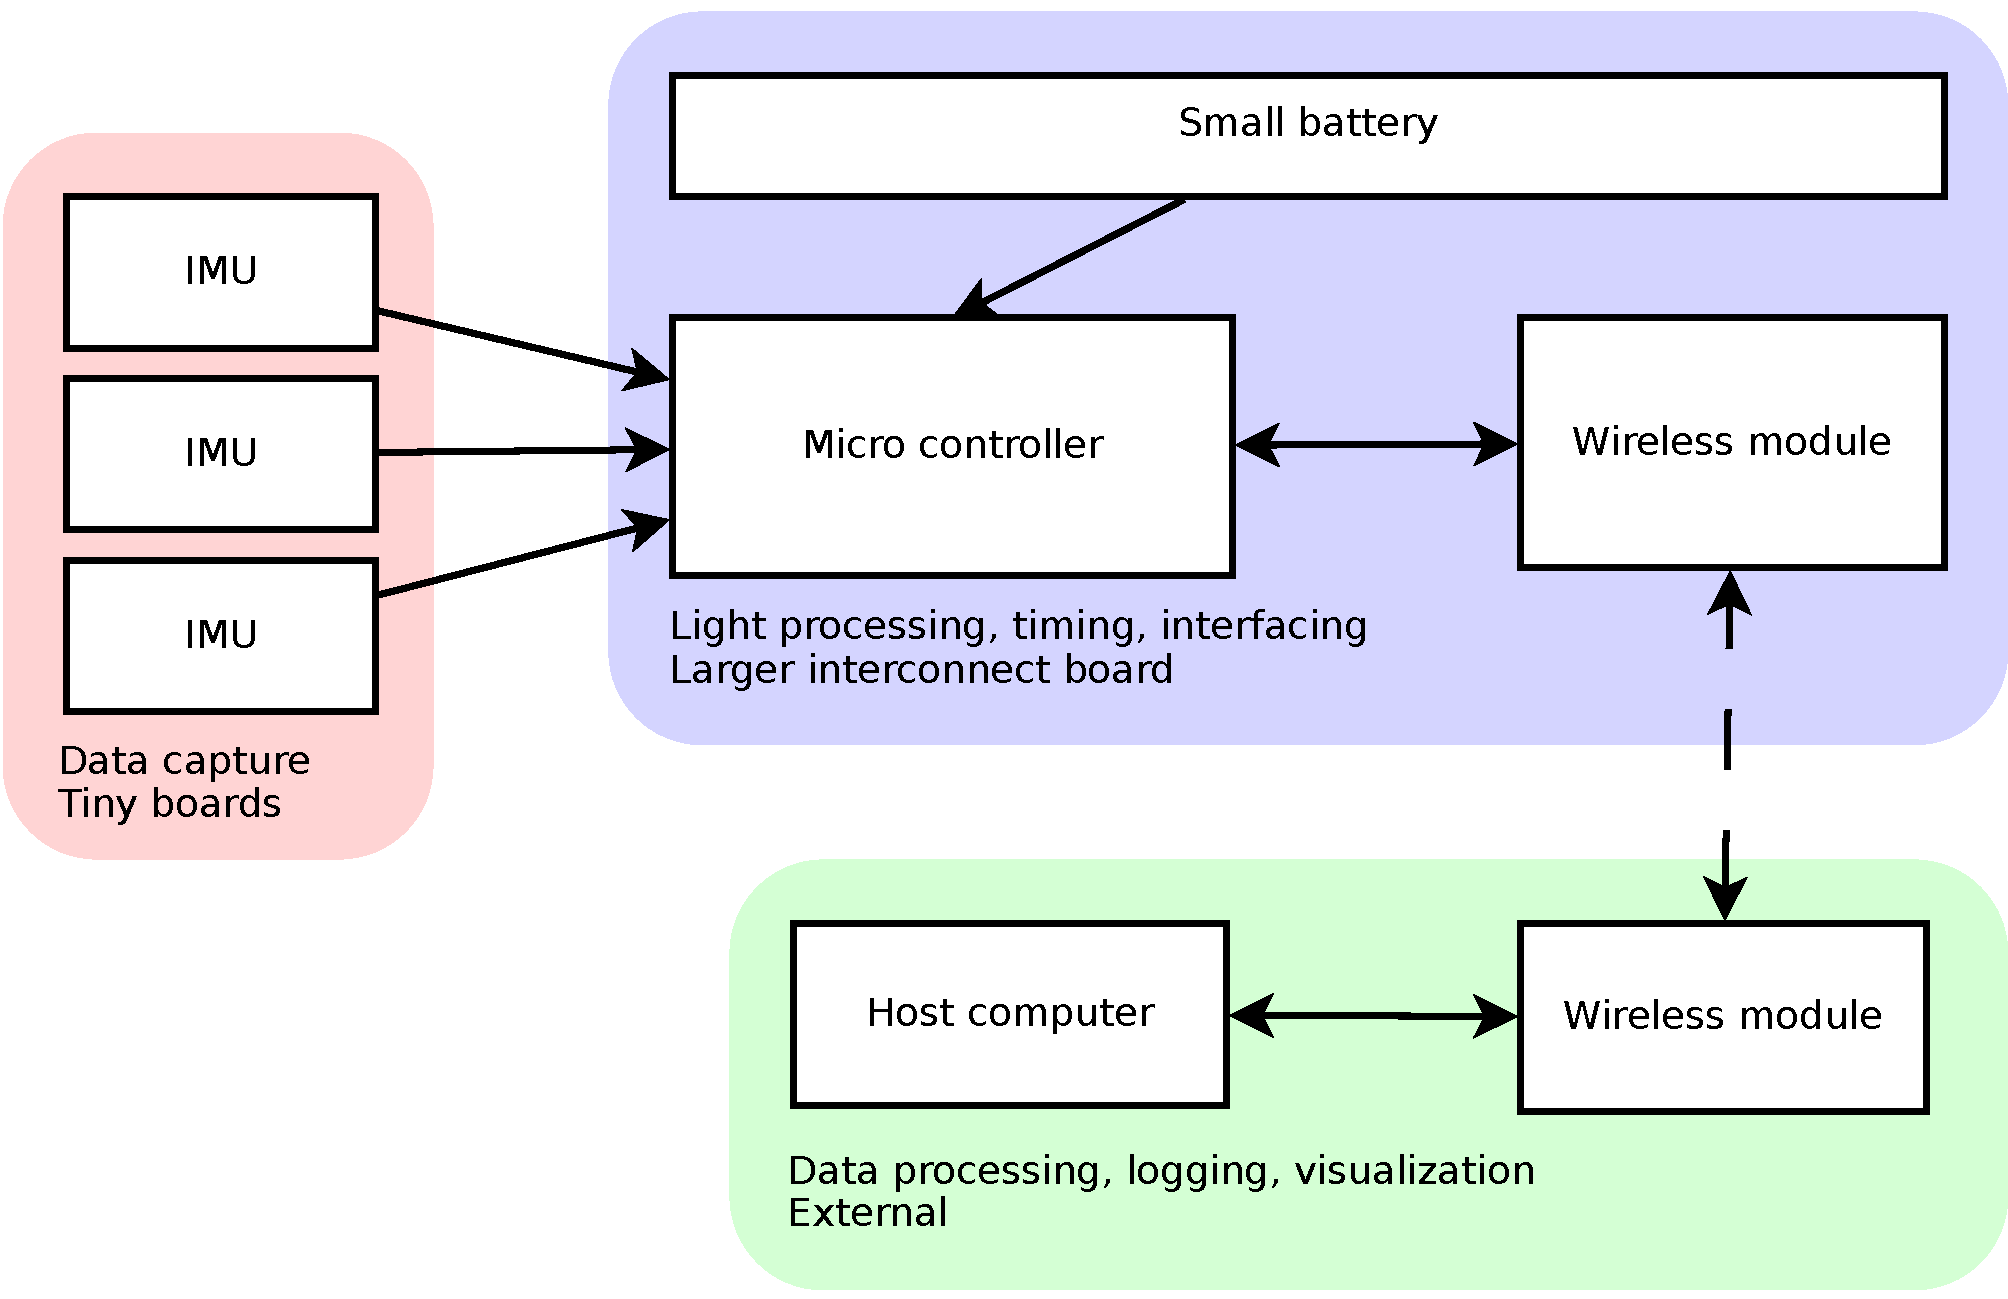
\includegraphics[scale=0.38]{block.pdf}
    \caption{A block diagram showing the most vital parts of the project, note that the different part is physically separeted.}
    \label{fig:pic2}
\end{figure}
\newpage

\subsection*{Software}
The software of this project can be described by the help of two flow charts, one representing the implementation on the motherboard and the other representing the host computer.

\subsubsection*{Micro controller software}
Figure~\ref{fig:pic3} shows how the motherboard application works in a comprehensive maner. In short the program first initializes the radio link and its communication protocol. 

The second step is to check and enumerate the number of IMUs that is connected to the motherboard. After initialization the soft ware enters a main loop where each IMU is sampled and the data is packed. If all samples have been taken then the data is transmitted to the host computer and the program goes back to the beginning of the loop and samples data from the IMUs again.    

\begin{figure}[h!]
    \centering
    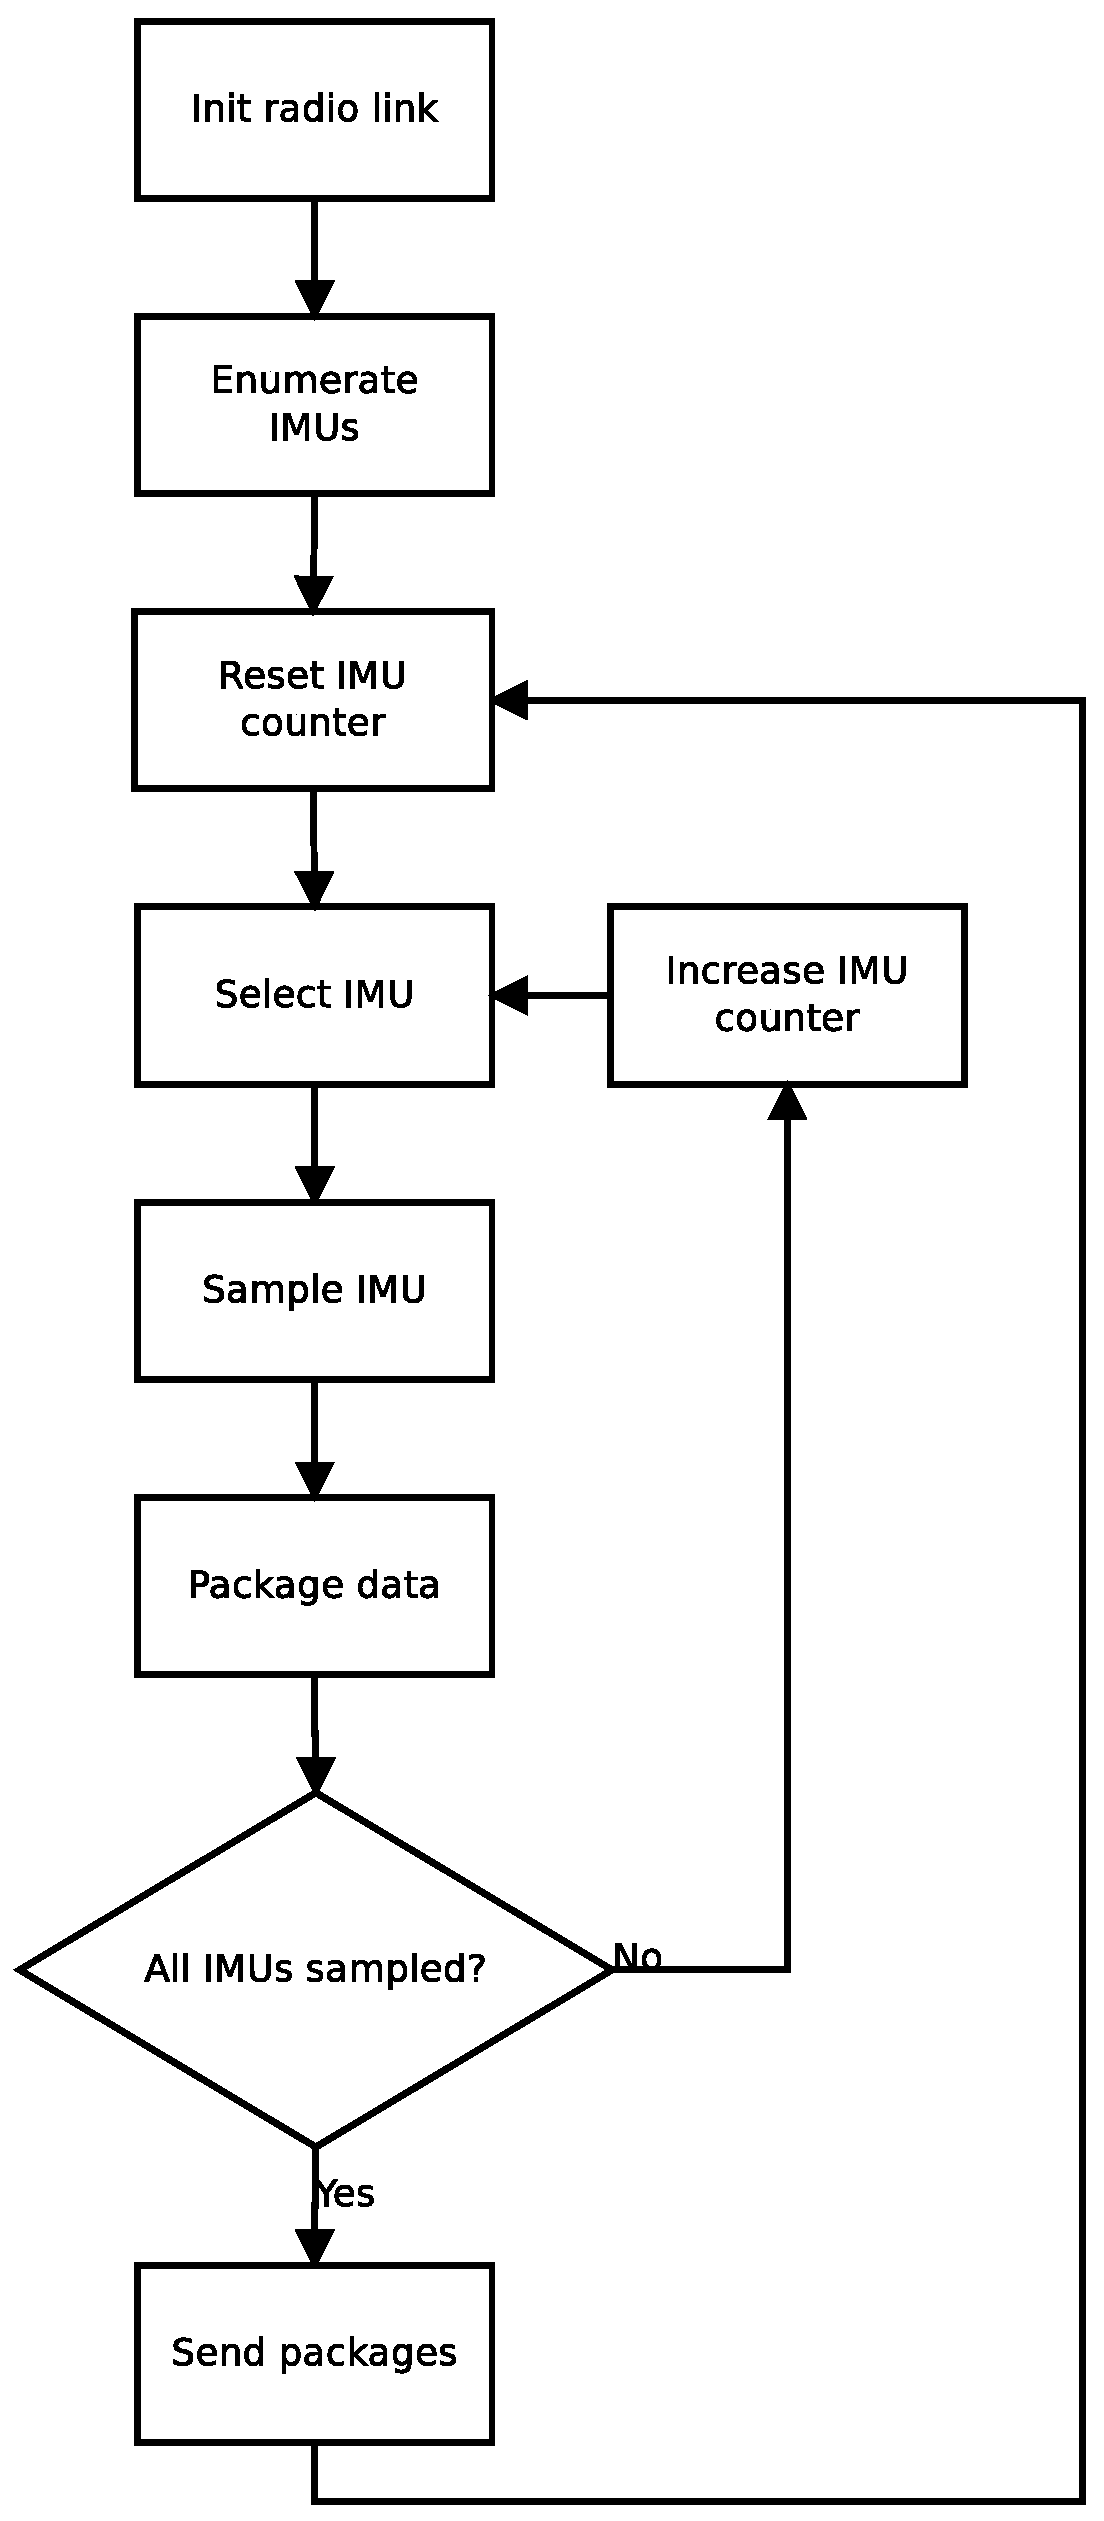
\includegraphics[scale=0.38]{micro.eps}
    \caption{A flow chart of motherboards micro controller code}
    \label{fig:pic3}
\end{figure}

\subsubsection*{Host computer software}
Figure~\ref{fig:pic4} illustrates the program flow of the host computer software.
The flow chart of the host computer is a bit more advanced and consists of several steps. The application begins by initializing the radio link and the skeleton structure from a pre-defined set of data points describing the spatial relation of the IMUs. After the initialization steps the program waits for data from the motherboard and when it is recieved the gyros are calibrated with regards of the gravity vector acquired from the accelerometers. The program then recalculates the bone structure, moving joints and rotating the limbs according to the sensor input.

In the main loop of the code, data is first read from the motherboard using the radio link. The relative rotational  from the gyros (angular speed) is integrated with respect to time. To mitigate the effects of gyro drift, the system constantly recalibrates itself. This is achieved by using the gravitational force acting upon the accelerometers as an absolute reference in space. However, since other forces act upon the accelerometer, some filtering is done to get better calibration. The accelerometer data is averaged over several (20) cycles and gravity data points from the accelerometer are only collected if the length of the accelerometer vector is close to 1G and the angular distance between the accelerometer vector and the supposed (calculated using gyros) gravity vector is small.

\begin{figure}[h!] %% För att H ska funka krävs väl float packetet?
    \centering
    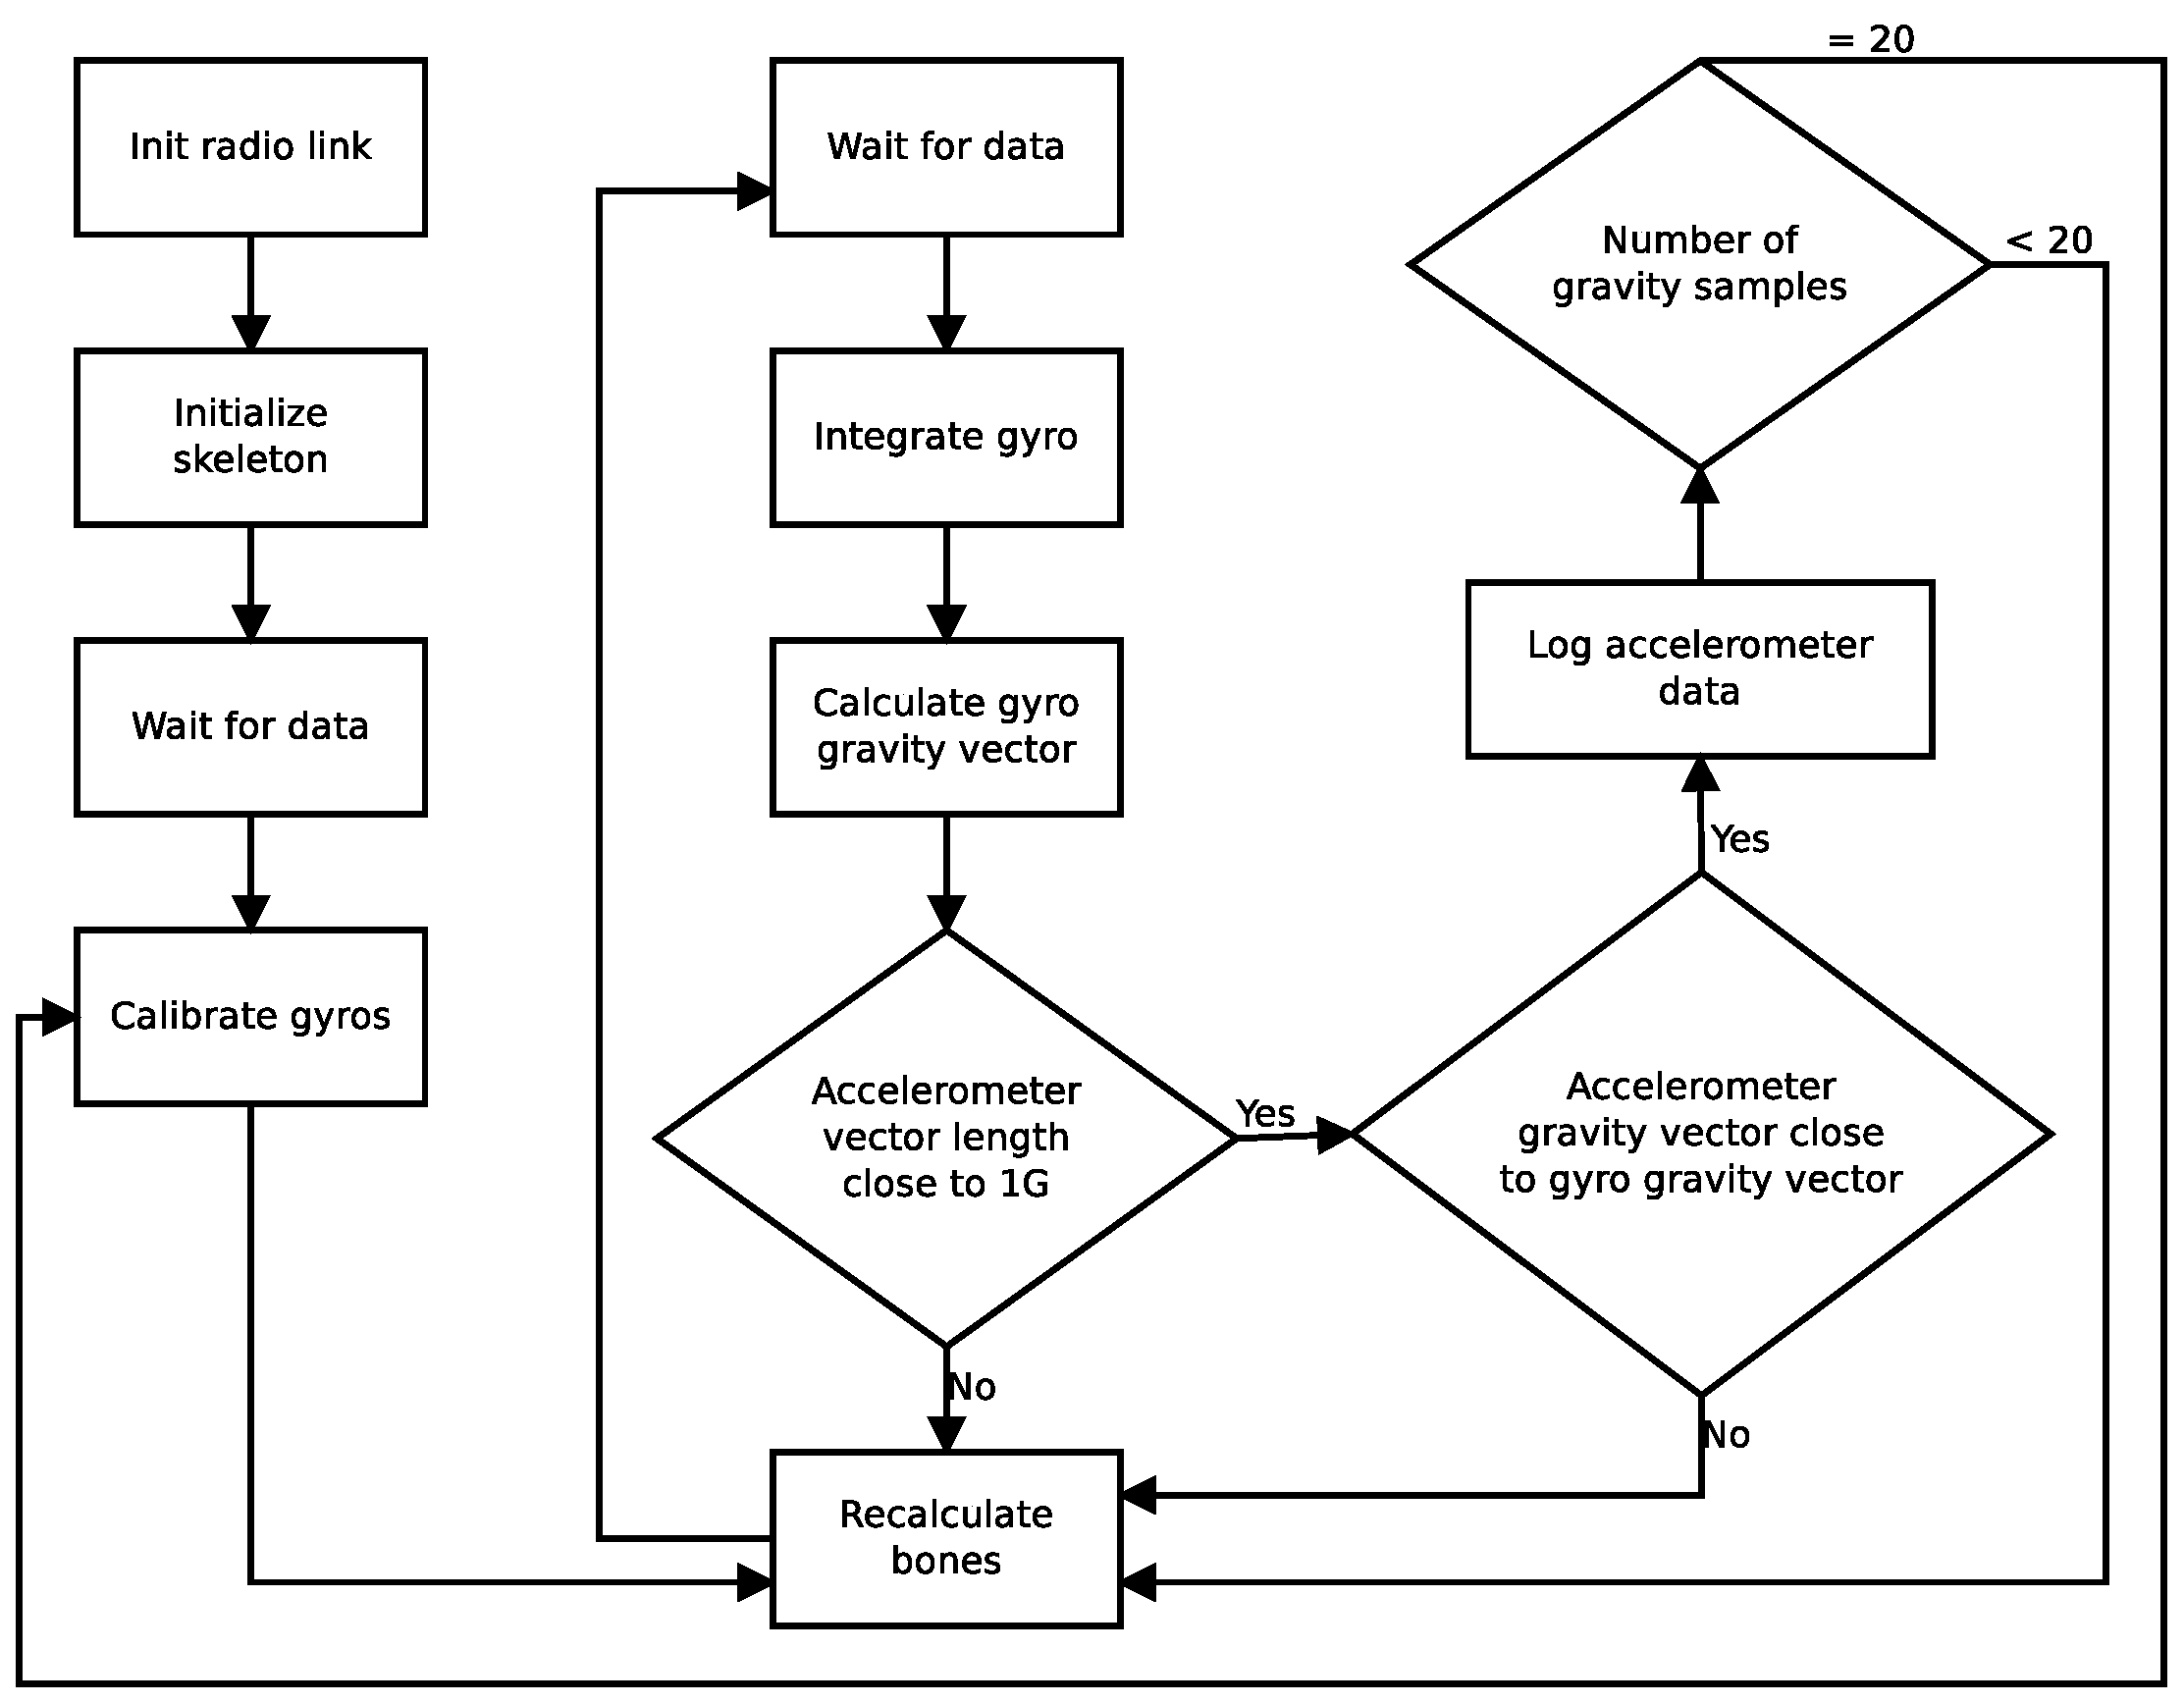
\includegraphics[scale=0.38]{pi.eps}
    \caption{Flow chart of host computer code}
    \label{fig:pic4}
\end{figure}

\subsection*{Hardware} % Ska vi ha med ngt om ritningarna till svarvade kretskort?
The hardware schematics of the system describes how it was constructed and the different components used. To make the system more reliable, robust and efficient the components where mounted on printed circuit boards designed during the course. Figure~\ref{fig:pic5} shows the schematics for the motherboard.
 

\begin{figure}[h!] %% Behöver nog kanske krympas lite 
    \centering
    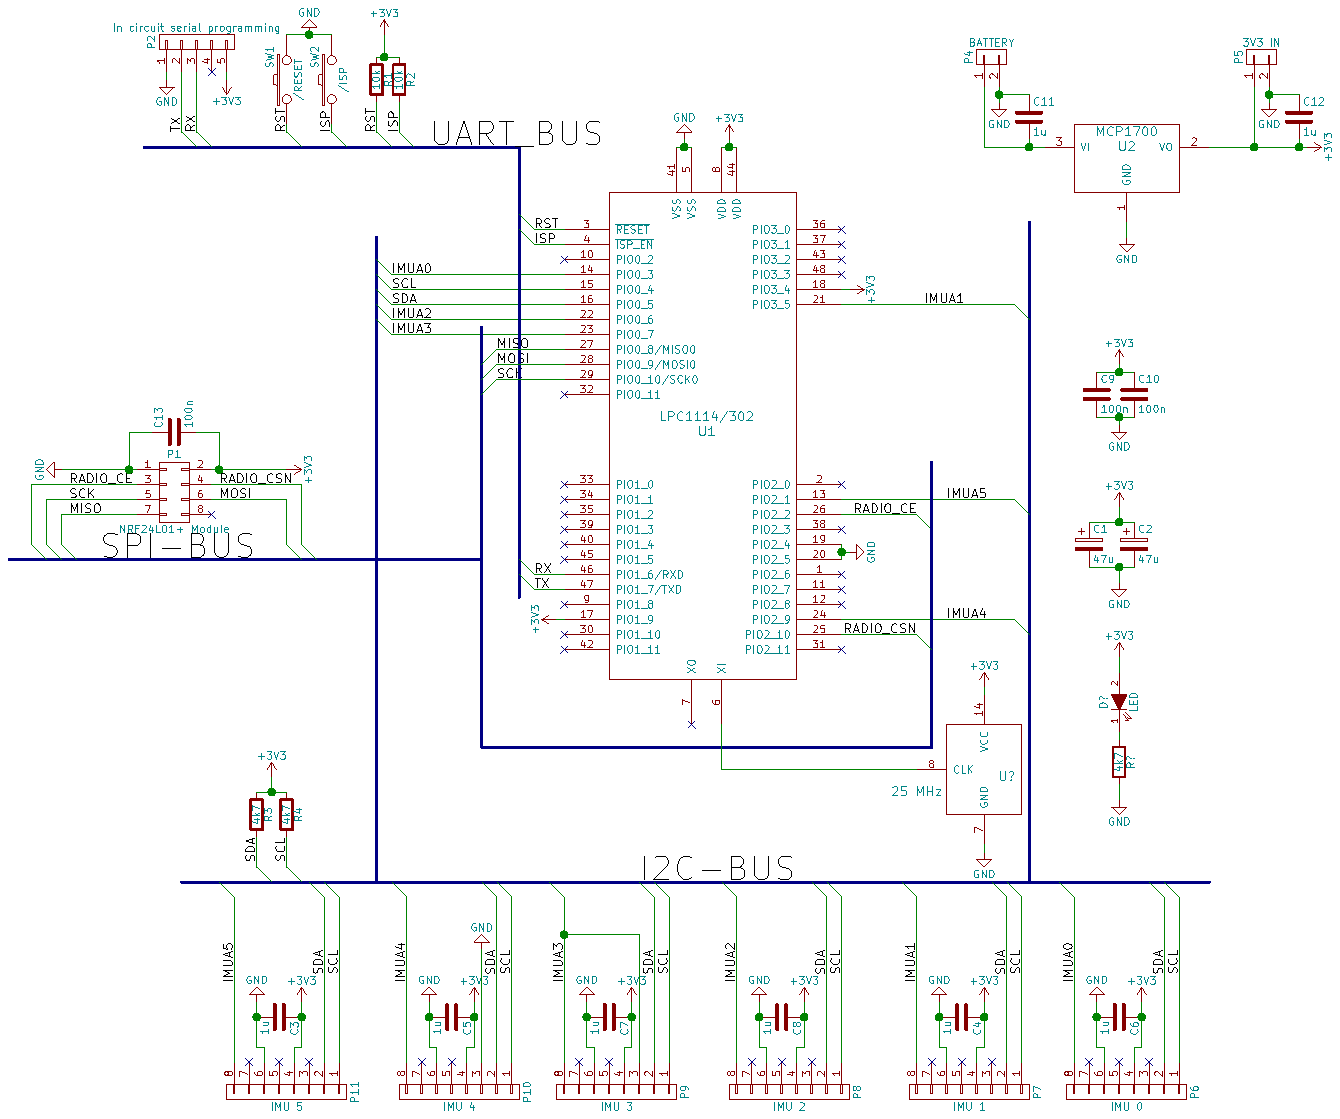
\includegraphics[scale=0.67]{mb_schematic.pdf}
    \caption{The Motherboard schematic}
    \label{fig:pic5}
\end{figure}

\noindent %lat
The connectors \textit{IMU 0} to \textit{IMU 5} on the motherboard (see Figure~\ref{fig:pic5}) will be connected to the \textit{CONN\_IN} connector on the different IMUs in the system. The IMU design are described by the schematics in Figure~\ref{fig:pic6} below. Note that the IMUs were constructed in a relativly small format which improved mobility but caused difficulties during the construction phase. % sista kanske lite överflödigt   
 
\begin{figure}[h!]%% För att H ska funka krävs väl float packetet?
    \centering
    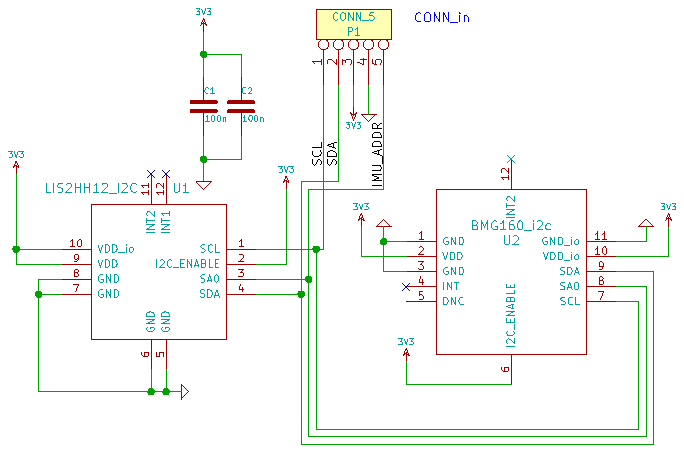
\includegraphics{imu_schematic.pdf}
    \caption{IMU board schematic}
    \label{fig:pic6}
\end{figure}


\section*{Data and Performance}
In this section of the report all the data and results of the project will be presented and evaluated. The measurements made have been focusing on capturing the system's drift over time and ability to correctly detect angles, both in high and low speed.

To collect data samples the system was installed in a simple laboration setup where angles could be read from the motion capturement system and a protractor. By reading values from a camera time could also be captured and measurements could be done in high speed. 

The setup was constructed by office-material found in the sourroundings to the project (see Figure~\ref{fig:pic7}), a folder was just as a hinge/joint and was stabilized by several books. A protractor was taped in line with the joint and made it possible to read angles manually. 

\begin{figure}[h!]
    \centering
    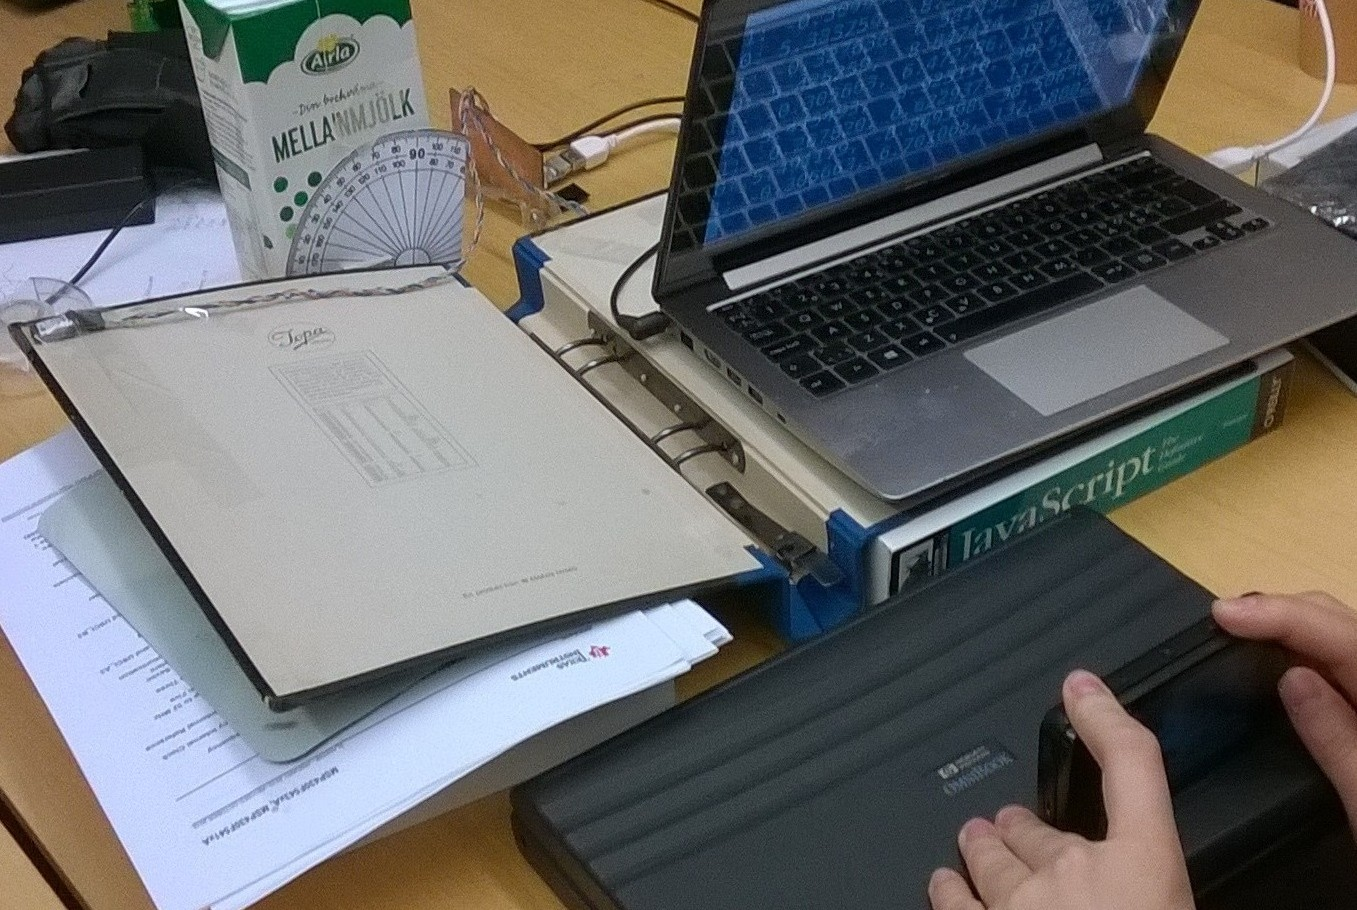
\includegraphics[scale=0.27]{croped.jpg}
    \caption{The laboration setup during data sampling for angles, note that the computer displays data values visible from the camera}
    \label{fig:pic7}
\end{figure}

To collect drift data of the system it was mounted on a table (which wasn't used) and then left to run for some time. During the execution data samples of the drift was taken and logged to make sure the drift is captured.     

\begin{figure}[h!]
    \centering
    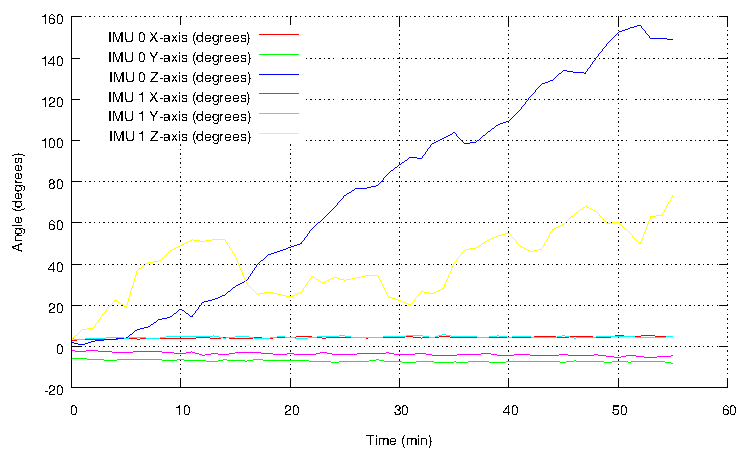
\includegraphics[scale=1.15]{drift.pdf}
    \caption{Stationary IMU drift over time}
    \label{fig:pic8}
\end{figure}

\begin{figure}[H]
    \centering
    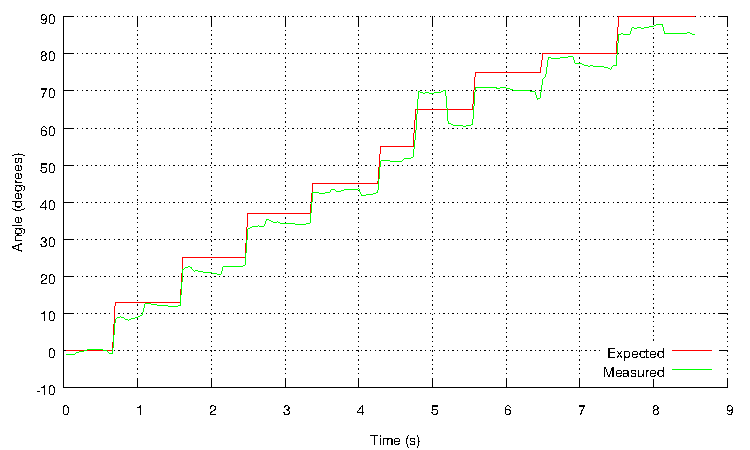
\includegraphics[scale=1.15]{stepped.pdf}
    \caption{Slow, stepped angle bend}
    \label{fig:pic8}
\end{figure}

\begin{figure}[H]
    \centering
    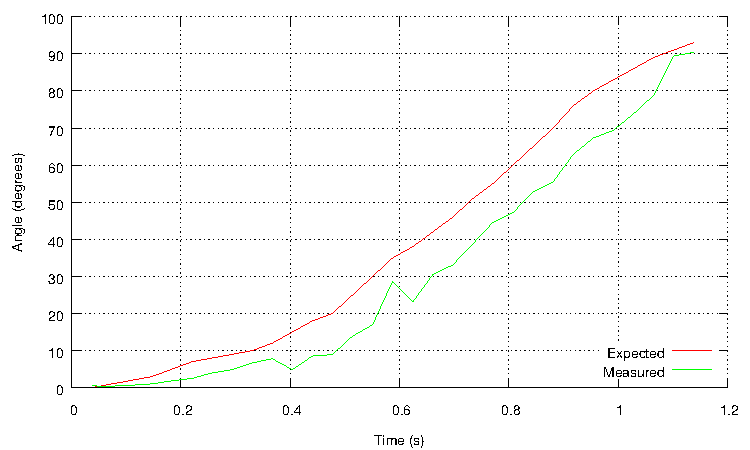
\includegraphics[scale=1.15]{fast_continuous.pdf}
    \caption{Fast, continuous bend}
    \label{fig:pic9}
\end{figure}

\section*{Individual reflection and Conclusion}


%%%%%%%%%%%%%%%%%%%%%%%%%%%%%%
%\newpage
%%\raggedright


\begin{thebibliography}{7}

\bibitem{kursp}
	The course web page,
	\url{https://people.kth.se/~msmith/II2302\_2016.html}, fetched \date{\today{}}.

\bibitem{wiki}
	Motion Capture on Wikipedia,
	\url{http://en.wikipedia.org/wiki/Motion\_capture}, fetched \date{\today{}}.

\bibitem{mems}
	MEMS on Wikipedia,
	\url{http://en.wikipedia.org/wiki/MEMS}, fetched \date{\today{}}.


\bibitem{accelerometer}
        LIS2HH12 accelerometer datasheet, ST Microelectronics, fetched \date{\today{}}
        \url{http://www.st.com/web/en/resource/technical/document/datasheet/DM00096789.pdf}
	
\bibitem{gyro}
        BMG gyro datasheet, Boch Sensortec, fetched \date{\today{}}
        \url{https://ae-bst.resource.bosch.com/media/products/dokumente/bmg160/BST-BMG160-DS000-09.pdf}
	

\end{thebibliography}
\end{document}

